\documentclass[a4paper,twoside,12pt]{article}

%the preamble
\usepackage[]{geometry}
\geometry{
	total={155mm,257mm},
	left=20mm,
	top=20mm,
}

\usepackage{marginnote}


\usepackage{lipsum}                     % Dummytext
\usepackage{xargs}    
\usepackage{amsmath,amsfonts,mathabx}
\usepackage{epigraph}  


\usepackage{framed}
\usepackage{color}

\newenvironment{shadequote}%
{\begin{snugshade}\begin{quote}}
		{\hfill\end{quote}\end{snugshade}}


\definecolor{shadecolor}{rgb}{0.9,0.9,0.9}






%\epigraphfontsize{\small\itshape}
%\setlength\epigraphwidth{10cm}
\setlength\epigraphwidth{.8\textwidth}
\setlength\epigraphrule{0pt}


%#this make the epigraph box with italic text
\usepackage{etoolbox}
\makeatletter
\newlength\epitextskip
\pretocmd{\@epitext}{\em}{}{}
\apptocmd{\@epitext}{\em}{}{}
\patchcmd{\epigraph}{\@epitext{#1}\\}{\@epitext{#1}\\[\epitextskip]}{}{}
\makeatother







% Use more than one optional parameter in a new commands
\usepackage[pdftex,dvipsnames]{xcolor}  % Coloured text etc.
% 
\setlength{\marginparwidth}{2cm}
\usepackage[colorinlistoftodos,prependcaption,textsize=tiny]{todonotes}
\newcommandx{\unsure}[2][1=]{\todo[linecolor=red,backgroundcolor=red!25,bordercolor=red,#1]{#2}}
\newcommandx{\change}[2][1=]{\todo[linecolor=blue,backgroundcolor=blue!25,bordercolor=blue,#1]{#2}}
\newcommandx{\info}[2][1=]{\todo[linecolor=OliveGreen,backgroundcolor=OliveGreen!25,bordercolor=OliveGreen,#1]{#2}}
\newcommandx{\improvement}[2][1=]{\todo[linecolor=Plum,backgroundcolor=Plum!25,bordercolor=Plum,#1]{#2}}
\newcommandx{\thiswillnotshow}[2][1=]{\todo[disable,#1]{#2}}
%

\usepackage{blindtext} % for dummy text
% \usepackage[margin=2cm]{geometry}   % to change margins
% \usepackage{titling}             % Uncomment both to   
% \setlength{\droptitle}{-2cm}     % change title position 







%%%%%%%%%%%%%%%%%%%%%%%%%%%%%%%%%%%%%%%%%%%%%%%%%%%%%%%%%%%%%%%%%%%%%%%%%%%%%%%%%%%


%       Document to Start HERE


%%%%%%%%%%%%%%%%%%%%%%%%%%%%%%%%%%%%%%%%%%%%%%%%%%%%%%%%%%%%%%%%%%%%%%%%%%%%%%%%%%%
\author{Nam Le}
\title{%\vspace{-1.5cm}            % Another way to do
	Balanced Scorecard for DUMMIES - A Summary}

%%%%%%%%%%%%%%%%%%%%%%%%%%%%%%%%%%%%%%%%%%%%%%%%%%%%%%%%%%%%%%%%%%%%%%%%%%%%%%%%%%%%


\begin{document}
\maketitle

\pagestyle{empty}

\section{Goals, Scores, and the Balanced Scoredcard}
\marginnote{The Balanced Scorecard was first developed
	in the early 1990s by two guys at the Harvard Business School: Robert
	Kaplan and David Norton}[1cm]

\begin{figure}[!htb]
	\centering
	%	\includepdf[angle = 0]{sections/CHE_1PHSC_with_VFD.pdf}
	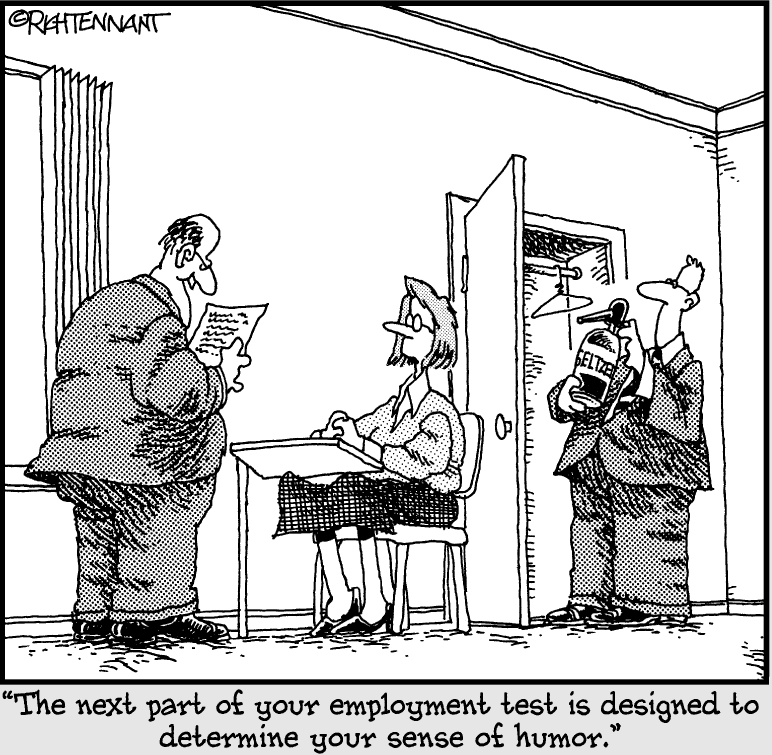
\includegraphics[scale=1.5]{figures/balancedscorecard_sensofhumor} \\
	%	\caption{Strategic management process}
	\label{balancedscorecard_sensofhumor} 
\end{figure}

So, what is the Balanced Scorecard? In short, it’s a management system that
enables your organization to set, track and achieve its key business strategies
and objectives. Once the business strategies are developed, they are
deployed and tracked through what we call the Four Legs of the Balanced
Scorecard. These four legs are made up of four distinct business perspectives:
The Customer Leg, the Financial Leg, the Internal Business Process Leg,
and the Knowledge, Education, and Growth Leg.

\epigraph{If you’re not keeping score, you’re
	just practicing. If you ask us, truer words were never spoken — especially
	in today’s topsy-turvy business world. To make (and keep) your business a
	success, you need to not only keep score, but also predict your score in advance
	by setting goals and then achieving them on a consistent basis. And we’re not
	talking about easy-to-achieve goals and scores. No! We’re talking about goals
	that stretch your imagination and push your creativity and ingenuity to the
	limits — as well as the creativity and ingenuity of your employees.}{}

\epigraph{Balanced
	Scorecard is a management system — not a measurement system. Yes, measurement
	is a key aspect of the Balanced Scorecard, but it is much more than
	just measurement: it is a means to setting and achieving the strategic goals
	and objectives for your organization.}{}









\end{document}
